\subsection{Application}
The application is implemented in the Angular framework using typescript as programming language. Typescript is a type-strong extension of the javascript language. The app is available at: \href{https://iottech18.herokuapp.com/}{https://iottech18.herokuapp.com/} The single page application is served from the server's main entry point. The application calls the API services as AJAX calls feeding the views with data. \\

The app presents all the sensor telemetry data live to the user, it manages device settings by updating threshold values and it monitor the device state and alerts. The app has three main views.
Figure \ref{fig:chartview} draws a live chart of incoming sensor telemetry. 

\begin{figure}[H]
    \centering
    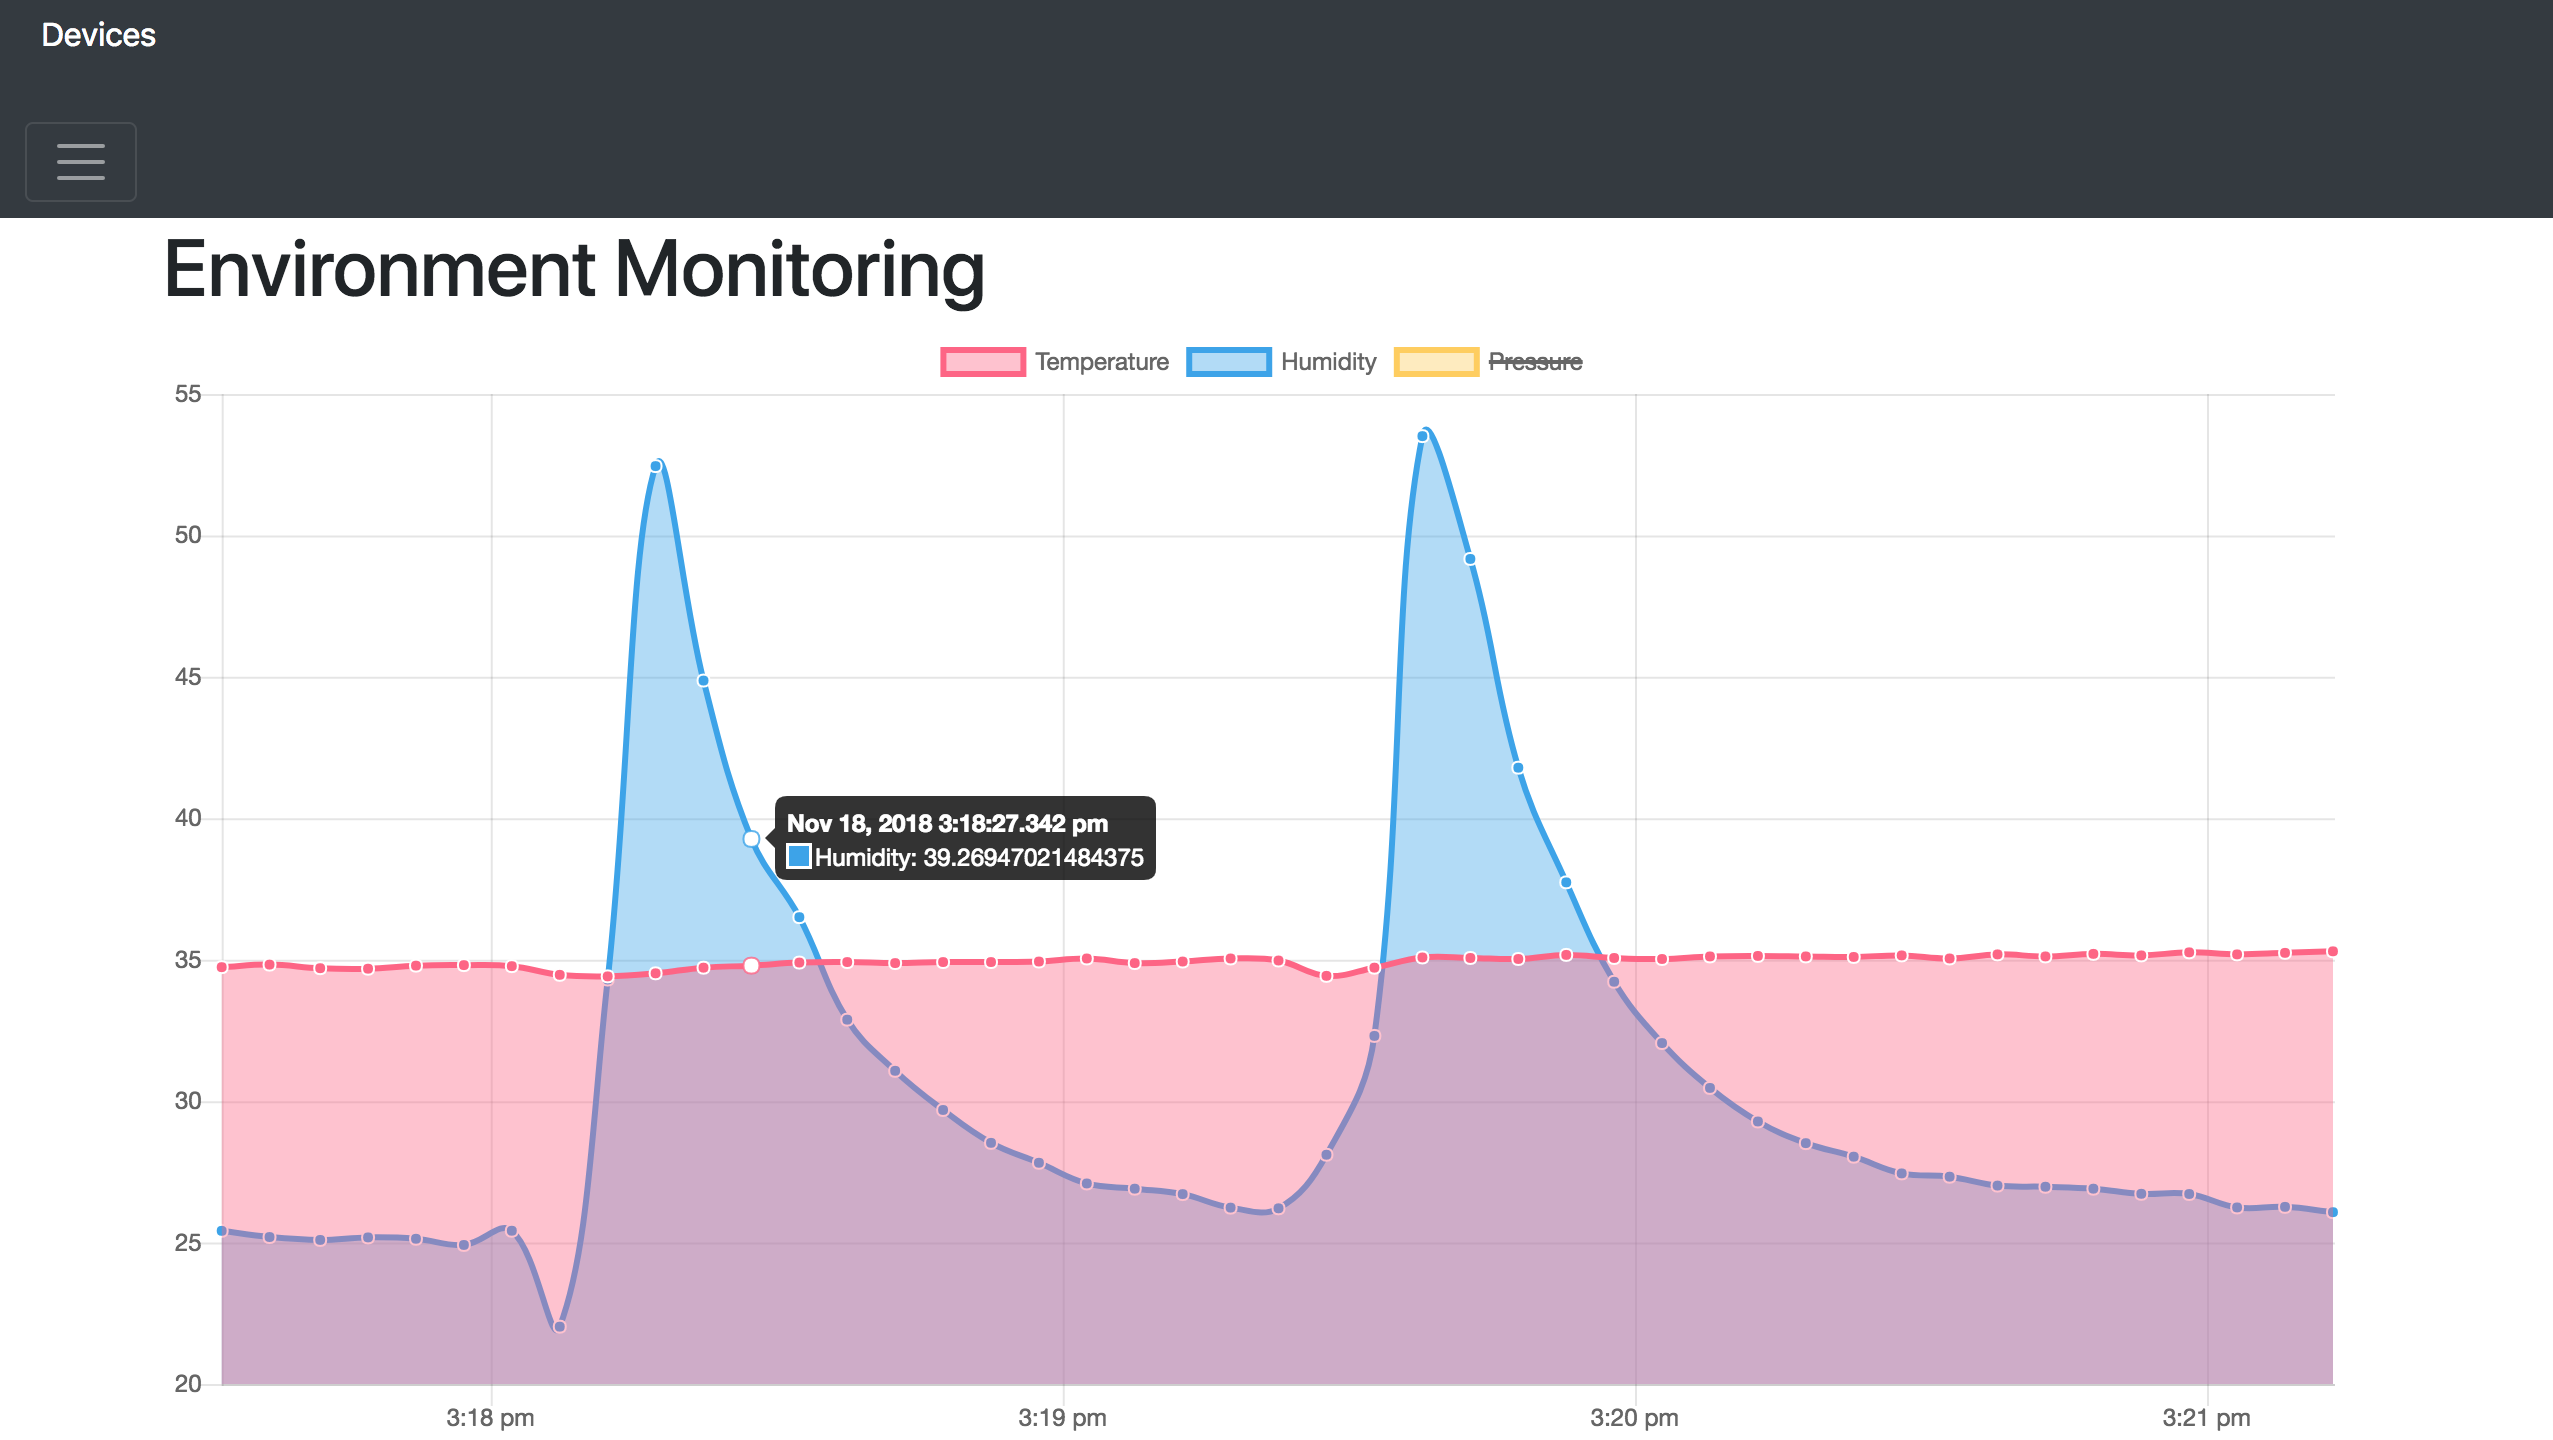
\includegraphics[width=0.9\textwidth]{figures/App/app_dashboard}
    \caption{Telemetry Chart View}
    \label{fig:chartview}
\end{figure}

Figure \ref{fig:devicelist} shows a list of all devices managed by the user. 

\begin{figure}[H]
    \centering
    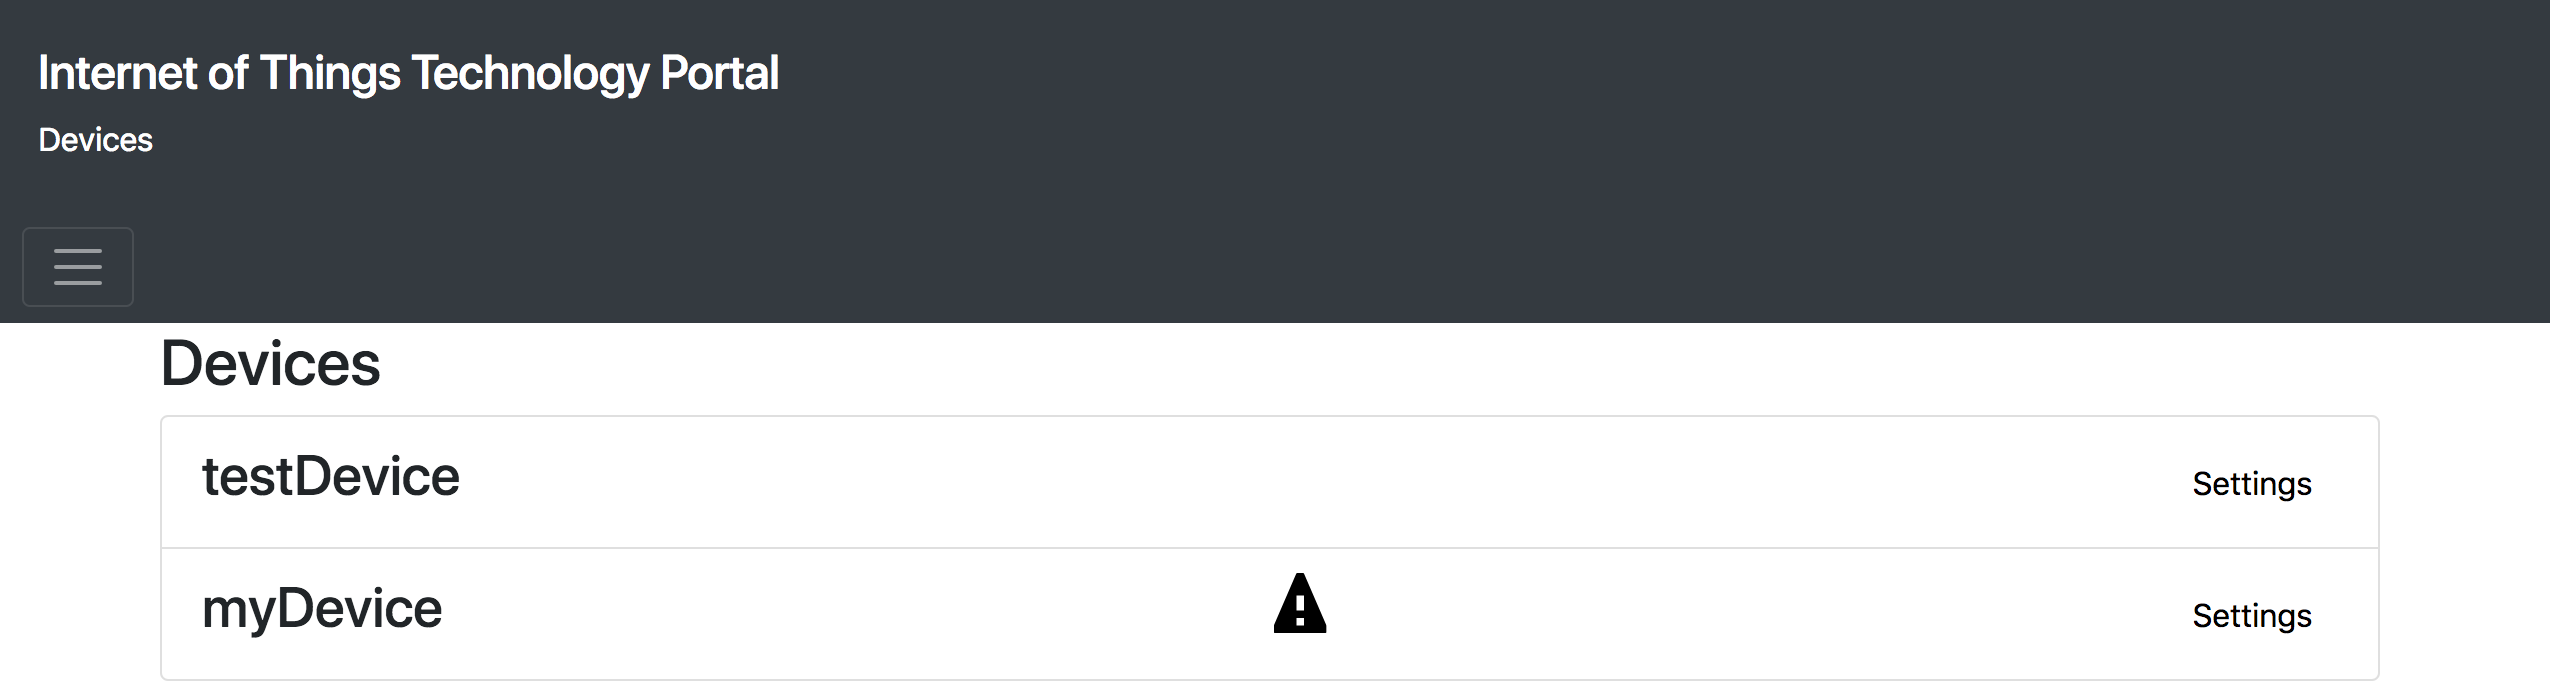
\includegraphics[width=0.9\textwidth]{figures/App/app_device_list}
    \caption{List of devices managed}
    \label{fig:devicelist}
\end{figure}

Figure \ref{fig:deviceoverview} shows the state of the device, the threshold it monitors and the alerts raised by the device monitored in real-time.

\begin{figure}[H]
    \centering
    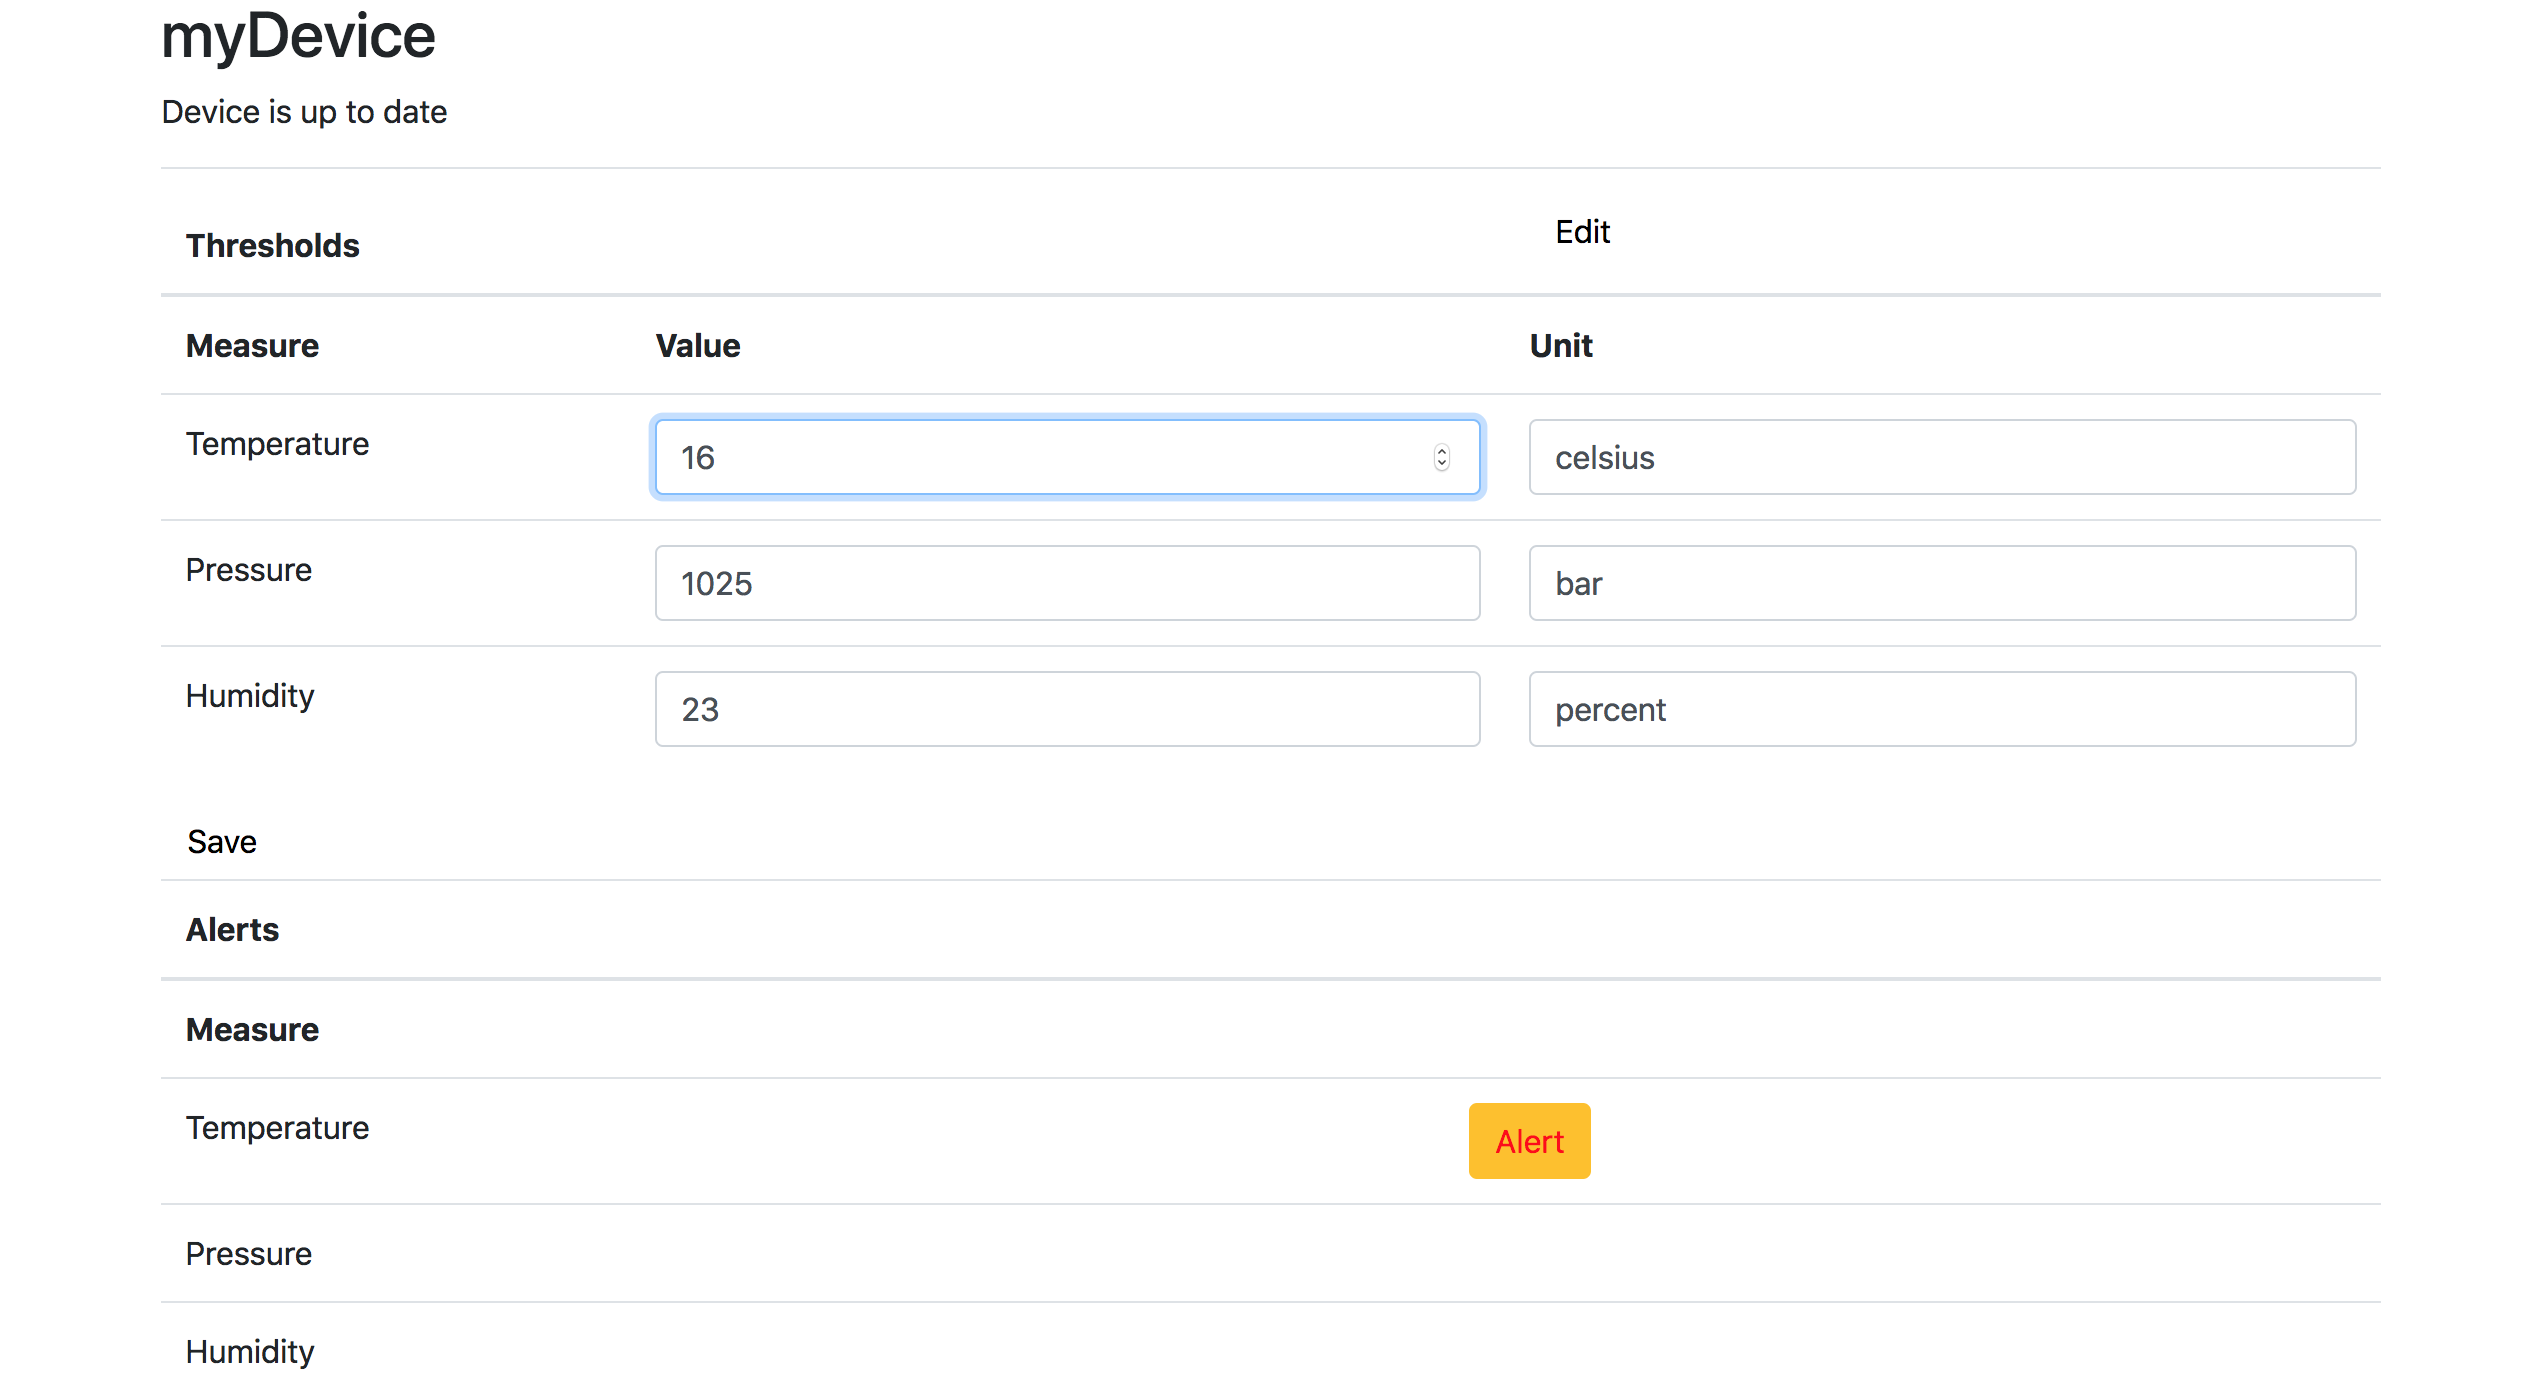
\includegraphics[width=0.9\textwidth]{figures/App/app_device_settings}
    \caption{Device state overview: Manage thresholds and monitors alerts}
    \label{fig:deviceoverview}
\end{figure}

The app subscribes to the server-sent-event by constructing an Event Source with an event listener, see listing \ref{lst:es}

\begin{lstlisting}[language=Python, caption=Event Source, label={lst:es}]
    this.source = 
        new EventSource('http://localhost:3000/api/telemetry/stream');
    this.source.addEventListener('message', event => {
      ...
      }
    )
\end{lstlisting}

The event listener adds the received telemetry data to the data structures holding prior telemetry received from an API request, as shown in listing \ref{lst:apirequest}. 


\begin{lstlisting}[language=Python, caption=API Request, label={lst:apirequest}]
    getAllTelemetry(): Observable<any> {
        return this.http.get(this.telemetryUrl);
      }
\end{lstlisting}